\documentclass[12pt]{article}

\usepackage{times,mathptmx}
\usepackage[pdftex]{graphicx}
\usepackage{pdflscape}

\usepackage{subcaption}
\usepackage{graphicx}
\usepackage{float}
\usepackage[section]{placeins}
\usepackage{fancyhdr}
\usepackage{enumitem}

\usepackage{xcolor}
\usepackage{listings}
\usepackage{textcomp}
\definecolor{lbcolor}{rgb}{0.96,0.96,0.96}
\lstset{
    backgroundcolor=\color{lbcolor},
    tabsize=4,
    rulecolor=,
    language=Fortran,
        basicstyle=\footnotesize\ttfamily,
        upquote=true,
        aboveskip={\baselineskip},
        belowskip={\baselineskip},
        columns=fixed,
        extendedchars=true,
        breaklines=true,
        breakatwhitespace=true,
        frame=none,
        showtabs=false,
        showspaces=false,
        showstringspaces=false,
        identifierstyle=\ttfamily,
        keywordstyle=\color[rgb]{0,0,0},
        commentstyle=\color[rgb]{0,0,0},
        stringstyle=\color[rgb]{0,0,0},
}

\usepackage{tocloft}
\usepackage[nottoc,notlof,notlot]{tocbibind} % Put the bibliography and index in the ToC

\pagestyle{fancy}
\rhead{}
\lhead{}
\chead{}
\cfoot{Page \thepage}
%\renewcommand{\headrulewidth}{0.4pt}
\renewcommand{\footrulewidth}{0.4pt}

\usepackage{color}
\usepackage{amsmath}
\usepackage{multirow}
\definecolor{linknavy}{rgb}{0,0,0.50196}
\definecolor{linkred}{rgb}{1,0,0}
\definecolor{linkblue}{rgb}{0,0,1}

\usepackage{xr-hyper}
\usepackage[pdftex,
        colorlinks=true,
        urlcolor=linkblue,     % \href{...}{...} external (URL)
        citecolor=linkred,     % citation number colors
        linkcolor=linknavy,    % \ref{...} and \pageref{...}
        pdfproducer={pdflatex},
        pagebackref,
        pdfpagemode=UseNone,
        bookmarksopen=true,
        plainpages=false,
        verbose]{hyperref}

\setlength{\textwidth}{6.5in}
\setlength{\textheight}{9.0in}
\setlength{\topmargin}{0.in}
\setlength{\headheight}{0.in}
\setlength{\headsep}{0.1in}
\setlength{\parindent}{0.25in}
\setlength{\oddsidemargin}{0.0in}
\setlength{\evensidemargin}{0.0in}

\newcommand{\pp}{\prime\prime}

\begin{document}

\bibliographystyle{unsrt}
\thispagestyle{empty}

\begin{center}
{\bf\Large Guidelines for Participation in the MaCFP-3 Workshop} \\
{\large October 22, 2023\\Tsukuba, Japan}
\end{center}

\begin{figure}[h]
  \centering
  \includegraphics[width=6in]{../../../matl-db/Documents/FIGURES/MaCFP_Logo.pdf}
  \label{Cover_Image}
\end{figure}

\vfill

\begin{minipage}{0.25\textwidth}
\begin{figure}[H]
\includegraphics[width=1.8in]{../../../matl-db/Documents/FIGURES/IAFSSLogo.pdf}
\end{figure}
\end{minipage} \hfill
\begin{minipage}{0.65\textwidth}
\begin{flushright}
\begin{small}
{\bf The MaCFP Working Group Organizing Committee:} \\
{\footnotesize Benjamin Batiot (University of Poitiers, France); Morgan Bruns (St. Mary's University, USA); Simo Hostikka (Aalto University, Finland); Isaac Leventon (National Institute of Standards and Technology, USA); Yuji Nakamura (Toyohashi University of Technology, Japan); Pedro Reszka (Universidad Adolfo Ibáñez, Chile); Thomas Rogaume (University of Poitiers, France); Stanislav Stoliarov (University of Maryland, USA); Fabian Bränsström (University of Wuppertal)}\\
{\footnotesize Alexander Brown (Sandia National Laboratories, USA); Andres Fuentes (Universidad Técnica Federico Santa María, Chile); Michael Gollner (University of California, Berkeley, USA); Anthony Hamins (National Institute of Standars and Technology, USA); John Hewson (Sandia National Laboratories, USA); Naian Liu (University of Science and Technology of China, China); Randy McDermott (National Institute of Standards and Technology, USA); Bart Merci (Ghent University, Belgium); Arnaud Trouvé (University of Maryland, USA); Yi Wang (FM Global, USA); Beth Weckman (University of Waterloo, Canada)}


\end{small}
\end{flushright}
\end{minipage}
\begin{small}
Document Prepared: March 9, 2023\\
\end{small}
\newpage
\thispagestyle{empty}
\tableofcontents

%\mainmatter
\pagestyle{empty}
\newpage
\section{Background}
\label{Sec:Background}
\subsection{MaCFP Working Group Motivation}
The general objective of the ``IAFSS Working Group on Measurement and Computation of Fire Phenomena" (abbreviated as the ``MaCFP Working Group") is to establish a structured effort in the fire research community to make significant and systematic progress in fire modeling, based on a fundamental understanding of fire phenomena. This is to be achieved as a joint effort between experimentalists and modelers, identifying key research topics of interest as well as knowledge gaps, and thereby establishing a common framework for fire modeling research. The spirit in which discussions will be conducted is collaborative and collegial.

The MaCFP Working Group is intended as an open, community-wide, international collaboration between fire scientists. It is also intended to be a regular series of workshops. The first MaCFP workshop~\cite{brown2018proceedings} was held on June 10-11, 2017, as a pre-event to the 12th IAFSS Symposium in Lund, Sweden. The second MaCFP workshop was held on April 22-23, 2021, as a pre-event to the 13th IAFSS Symposium. Details on the content and outcomes of the first and second MaCFP workshops (called MaCFP-1 and MaCFP-2) can be found on the MaCFP website (\url{https://iafss.org/macfp/}) and MaCFP repository (\url{https://github.com/MaCFP}). Presentations for the first two MaCFP workshops can be found on the GitHub Releases pages:
\begin{itemize}[noitemsep]
 \item \href{https://github.com/MaCFP/macfp-db/releases/tag/macfp-1.0}{MaCFP-1 (Lund, 2017)}
 \item \href{https://github.com/MaCFP/macfp-db/releases/tag/macfp-2.0}{MaCFP-2 (Waterloo, 2021) - Gas Phase}
 \item \href{https://github.com/MaCFP/matl-db/releases/tag/v1.1.0}{MaCFP-2 (Waterloo, 2021) - Condensed Phase}
\end{itemize}

MaCFP target experiments correspond to basic configurations (building blocks) with carefully-controlled conditions and quality instrumentation and diagnostics. The initial list of target experiments included turbulent buoyant plumes, turbulent pool fires (gaseous and liquid fuels), gaseous wall fires, and flame extinction; each case corresponds to openly-available databases. This list will be enhanced as the MaCFP Working Group makes progress and moves towards greater complexity and realism. At MaCFP-3, a new category will be presented and studied: Fire Growth.

The specific objectives of the MaCFP Working Group are to:
\begin{itemize}[noitemsep]
 \item Develop a digital archive of well-documented fire experiments that can be used as targets for CFD model validation;
 \item Develop a digital archive of well-documented CFD-based numerical simulations corresponding to the selected target experiments;
 \item Develop protocols for detailed comparisons between computational results and experimental measurements;
 \item Identify key research topics and knowledge gaps in computational and experimental fire research;
 \item Develop best practices in both computational and experimental fire research (including quality control and quantification of uncertainties);
 \item Establish a network between fire researchers and provide a community-wide forum for discussion and exchange of information.
\end{itemize}



\subsection{The MaCFP Repository (Github)}
The MaCFP repository is hosted on GitHub (\url{https://github.com/MaCFP}). Note that the repository is continuously updated, and users are expected to consult the repository regularly for possible additions and/or corrections. This data repository is available to computational groups for fire model calibration and validation. The repository is managed by Randy McDermott and Isaac Leventon of the National Institute of Standards and Technology (NIST). It contains:
\begin{itemize}[noitemsep]
 \item A description of each selected target experiment, including a description of the experimental configuration and a description of measured quantities and measurement uncertainties (if known);
  \item A description of each selected target experiment, including a description of the experimental configuration and a description of measured quantities and measurement uncertainties (if known);
 \item An electronic copy of experimental data organized in simple comma-delimited ASCII files;
 \item An electronic copy of computational results submitted by the different modeling groups that participated in the MaCFP-1 and MaCFP-2 Workshops, also organized in simple comma delimited ASCII files;
  \item An electronic copy of material property sets (i.e., pyrolysis models) calibrated by the different modeling groups that MaCFP-2 Workshop, also organized in simple comma delimited ASCII files;
 \item Protocols to perform comparisons between experimental data and simulation results based on (provided) MATLAB-based post-processing tools.
 \item Copies of presentations (lecture slides and audio/video recordings) given at the MaCFP-1 and MaCFP-2 Workshops
\end{itemize}

This guidelines document provides a summary of specific modeling targets of interest for each target experiment to be presented at the MaCFP-3 Workshop. Participants can submit their contributions by creating a pull request on Github; details on how to do so (including file formatting requirements) are provided in Secs.~\ref{Sec:Gas Phase}-\ref{Sec:Com-Results}. Python-based \href{https://github.com/MaCFP/macfp-db/wiki/Plotting-Scripts}{post-processing tools are available} on the repository, thus, contributors need only to submit comma-delimited (*.csv) files with their computational results together with another comma-delimited configuration file listing the plots to be made\footnote{Participants submitting new or revised pyrolysis models (i.e., material property sets) are asked to provide further information, as described in Sec.~\ref{Sec:Pyrolysis}}. Further details on \href{https://github.com/MaCFP/macfp-db/wiki/How-to-Contribute}{how to contribute} and \href{https://github.com/MaCFP/macfp-db/wiki/Submitting-Computational-Results}{how to submit computational results} are available on the MaCFP-db wiki.  Please contact Randy McDermott (\href{mailto:randall.mcdermott@nist.gov}{randall.mcdermott@nist.gov}) if you have any questions regarding submission of results or post-processing.

\newpage
Interested modeling groups should inform the Gas Phase and Condensed Phase Phenomena subgroups of their plans to participate in MaCFP-3 by contacting the following Co-Chairs:

\begin{itemize}[noitemsep]
\item Morgan Bruns, \href{mailto:mbruns@stmarytx.edu}{mbruns@stmarytx.edu} (Co-Chair of the Condensed Phase Phenomena subgroup) (NIST-Gasification-Apparatus, UMD-SBI, NIST-Parallel-Panel)
\item Isaac Leventon, \href{mailto:isaac.leventon@nist.gov}{isaac.leventon@nist.gov} (Co-Chair of the Condensed Phase Phenomena subgroup) (NIST-Gasification-Apparatus, UMD-SBI, NIST-Parallel-Panel)
\item Bart Merci, \href{mailto:Bart.Merci@ugent.be}{Bart.Merci@ugent.be} (Co-Chair of the Gas Phase Phenomena subgroup) (NIST-Pool-Fires, FM-Burner, UMD-SBI, NIST-Parallel-Panel)
\item Arnaud Trouv\'e, \href{mailto:atrouve@umd.edu}{atrouve@umd.edu} (Co-Chair of the Phase Gas Phenomena subgroup) (NIST-Pool-Fires, FM-Burner, UMD-SBI, NIST-Parallel-Panel)
 \end{itemize}

Users of the experimental measurements and model parameters found in the Condensed Phase Material Database~\cite{MaCFP-cond-db} are encouraged to: (a) cite the repository (see below); (b) to cite related summary publications, if using the analysis results prepared in these documents (e.g., conference proceedings~\cite{brown2018proceedings} or the preliminary summary of experimental measurements document~\cite{MaCFP-2_Prelim_Exp}); and (c) to directly credit the institutions that provided experimental measurements (relevant publications and contributor information) are detailed in the README file associated with each institutional dataset.

The MaCFP Condensed Phase Github repository is version controlled. When citing this database, please include the date accessed. You may cite the use of this data as follows:

\begin{lstlisting}
Leventon, I., Batiot, B., Bruns, M., Hostikka, S., Nakamura, Y., Reszka, P., Rogaume, T., Stoliarov, S., Measurement and Computation of Fire Phenomena (MaCFP) Condensed Phase Material Database, https://github.com/MaCFP/matl-db, date accessed: day-month-year, https://doi.org/10.18434/mds2-2586.
\end{lstlisting}

\clearpage
\section{MaCFP-3: Tsukuba, Japan (2023)}
\label{Sec:MaCFP-3}
\subsection{Workshop Presentation Topics}
\label{Sec:MaCFP-3 Target Cases}
On Sunday, October 22, 2023, the third Measurement and Computation of Fire Phenomena Workshop (MaCFP-3) will be hosted (in-person) as a pre-event to the IAFSS meeting in Tsukuba, Japan. At this workshop, we will present new experimental measurements and numerical simulations focused on separate condensed- and gas-phase phenomena as well as our first ever coordinated attempt to model coupled condensed/gas phase cases: flame spread over a combustible solid (i.e., the reference material characterized as part of the MaCFP-2 Workshop). In addition, a new sub-group focusing on Radiation Heat Transfer Phenomena will be launched. It will focus on creating new radiation benchmark problems for the fire-related radiation problems in gas and condensed phase, and using them to improve the radiation sub models of the fire models.\\

MaCFP-3 target presentations include:
\begin{itemize}[noitemsep]
\item \href{https://github.com/MaCFP/macfp-db/tree/master/Liquid_Pool_Fires/NIST_Pool_Fires}{NIST-Pool-Fires}: 30 cm, 37 cm, and 100 cm diameter liquid pool and gaseous burners studied at NIST and featuring multiple fuels;
\item \href{https://github.com/MaCFP/macfp-db/tree/master/Extinction/FM_Burner}{FM-Burner}: 13.7 cm diameter ethylene diffusion flames studied at FM Global and featuring a controlled co-flow oxygen-nitrogen oxidizer;
\item \href{https://github.com/MaCFP/matl-db/tree/master/PMMA/Validation_Data/NIST_Gasification_Apparatus}{NIST-Gasification-Apparatus}: bench-scale thermal degradation experiments conducted in the NIST gasification apparatus, providing validation data for PMMA pyrolysis models;
\item \href{https://github.com/MaCFP/macfp-db/tree/master/Fire_Growth/UMD_SBI}{UMD-SBI}: Flame spread experiments in a 1.46 m corner wall configuration studied at the University of Maryland with MaCFP PMMA (based on the Single Burning Item (SBI) Test, EN13823~\cite{EN-13823standard});
\item \href{https://github.com/MaCFP/macfp-db/tree/master/Fire_Growth/NIST_Parallel_Panel}{NIST-Parallel-Panel}: Flame spread experiments in a 2.44 m parallel panel configuration studied at NIST with MaCFP PMMA (based on the FM4910 Parallel Panel Test~\cite{FM-4910standard}).
\end{itemize}


\subsection{Workshop Schedule}

The MaCFP-3 Workshop is tentatively scheduled to have two sessions (morning and afternoon, with a lunch break in between). This first half of the meeting will focus on target experiments (and related modeling) that have been organized separately by either the gas-phase or condensed-phase working groups (e.g., pool fires or determination of solid-phase material properties). The second half of the meeting will focus on coupled solid/gas phase experiments (i.e., fire growth over a combustible solid). In each session, an emphasis is maintained on providing time for open discussion among active participants of the working group in order to facilitate ongoing and future collaboration in this effort. A poster session will be organized for experimentalists and modelers to discuss current results and possible future target experiments. The workshop will be organized to allow substantial time for open discussion and interaction among participants.\\

Discussion topics may include:
\begin{itemize}[noitemsep]%,topsep=0pt
\item Guidelines for experimental calibration/description needs
\item Guidelines, needs, and/or knowledge gaps in pyrolysis/fire model verification and validation
\item Understanding fire model sensitivity to variability in pyrolysis model parameters
\item Pyrolysis model verification exercise for MaCFP-4
\item Identification of a new material of interest for MaCFP-4
\item Proposed new target cases for radiation heat transfer and gas-phase model validation
\item Frequency and locations of future MaCFP meetings and workshops (virtual + in person)
\end{itemize}


%\textbf{Morning Session}
%\begin{itemize}[noitemsep]
%\item (15 min) Welcome presentation
%\begin{itemize}[noitemsep]
%\item Experimental Setup, quality of measurement results
%\item Guidelines on modeling results (e.g., setup, grid/angular resolution, submodels...)
%\end{itemize}
%\item (35 min) Pool Fires (New measurements: multiple fuels, soot, gaseous species, radiation)
%\item (35 min) FM Gas burner
%\item (30 min) Launch of new Subgroup: Radiation Heat Transfer Phenomena
%\item (35 min) New PMMA validation case (1D Gasification experiments + revised pyrolysis property sets)
%\item (30 min) Open discussion, with targeted discussion topics:
%\begin{itemize}[noitemsep]
%\item New materials? ( using existing test framework)
%\item Defining standards for `good' experimental data and/or modeling results
%\item Creation of a third subgroup (radiation) and who would lead that effort
%\end{itemize}
%\end{itemize}
%
%\textbf{Lunch Break}\\
%
%\textbf{Afternoon Session}
%\begin{itemize}[noitemsep]
%\item (60 min) Single Burning Item tests (UMD)
%\begin{itemize}[noitemsep]
%\item (20 min) Experimental setup and measurements
%\item (20 min) Simulation results: summarize submodels used; highlight key results
%\item (20 min) Focused discussion
%\end{itemize}
%\item (60 min) Parallel panel tests (NIST)
%\begin{itemize}[noitemsep]
%\item (20 min) Experimental setup and measurements
%\item (20 min) Simulation results: summarize submodels used; highlight key results
%\item (20 min) Focused discussion
%\end{itemize}
%\item (60 min) Open discussion: next steps for MaCFP-4 (2026)
%\begin{itemize}[noitemsep]
%\item Can we repeat simulations with different pyrolysis models?
%\item Next simulation case (e.g., fundamentally new tests)?
%\item Pyrolysis model verification exercise for MaCFP-4
%\item Identification of a new material of interest for MaCFP-4
%\item Timeline of future MaCFP events, meetings, and workshops
%\end{itemize}
%\end{itemize}

\subsection{Timeline of Events in Preparation for MaCFP-3}

\label{Timeline}
\begin{table}[h!]
\begin{tabular}{p{0.25\linewidth} | p{0.7\linewidth}}
\hline
\textbf{Date}          & \textbf{Objective} \\
\hline
December 20, 2022      & Share call for participation in MaCFP-3\\
                       & Experimental Measurements (fire growth) added to repo\\
\\
March 10, 2023          & Share `Guidelines for Participation in MaCFP-3' document \\
                       & Modeling results from MaCFP-2 organized and added to Github Repo (simulations data + PMMA pyrolysis model parameters)\\
                       & Pyrolysis modeling validation dataset added to repo\\
\\
March 23, 2023         & Virtual meeting (all participants welcome)\\
12:30 PM (EST)         & Share new experimental data (NIST gasification apparatus); condensed-phase modelers are asked to perform:\\
                       & (a) Blind validation: Predict these new results based on their original pyrolysis model properties. \\
                       & (b) Recalibration: Adjust pyrolysis model parameters \textit{as needed} to provide better predictions (modelers must describe any changes made)\\
                       & Introduce MaCFP-3 gas-phase and coupled condensed- and gas-phase target cases\\
\\
June 1, 2023           & Condensed-phase modelers asked to prepare and submit final parameter sets and model predictions of: \\
                       & (1) New experimental data (NIST Gasification Apparatus)\\
                       & (2) Ideal gasification tests (Incident heat flux, $\dot{q}^{\pp}=$10, 25, 65 ~kW~m$^{-2}$; Sample thickness, 6~mm and 12~mm)\\
\\
Summer 2023           & Virtual Meeting  (all participants welcome):\\
                       & Present validation of pyrolysis model parameter sets based on new gasification data \\
                       & Preliminary analysis - relative impact on variability in final model predictions\\
\\
August 31, 2023        & Deadline to share flame spread modeling results \\ {}\\
October 22, 2023       & MaCFP-3 Workshop: Tsukuba, Japan \\
\hline
\end{tabular}
\end{table}

\clearpage
\section{Gas-Phase Modeling}
\label{Sec:Gas Phase}
Two experiments of gas-phase fire behavior (liquid pool fires \& gaseous burners, and a co-flow round diffusion flame) are provided for consideration in the MaCFP-3 Workshop.  Computational results submitted for each for these target experiments (as well as coupled condensed-and gas-phase fire growth simulations, see Sec.~\ref{Sec:Fire Growth}) should comply with the following series of requirements:

\begin{itemize}[noitemsep]
\item We ask that for each simulated target experiment, the submission includes a grid convergence study in which the effect of changing spatial resolution in the flow and combustion solver is quantified;
\item Similarly, we ask that for each simulated target experiment that includes heat flux measurements, the submission includes an angular convergence study in which the effect of changing angular resolution in the radiation solver is quantified;
\item We also ask that modeling groups explain their modeling choices for the treatment of the turbulent flow, combustion and radiation transport; we encourage modeling groups to define a baseline model and apply that model to all simulated cases considered by the group; and we ask that variations in modeling choices be justified.
 \end{itemize}

Modeling groups are encouraged to consider performing fine-grained simulations under the high-resolution conditions that are often the preferred choice made by CFD researchers, and also consider performing coarse-grained simulations under the moderate-to-marginal resolution conditions (sometimes called VLES) that are more representative of the choices made by CFD practitioners.

\subsection{NIST-Pool-Fires}
\href{https://github.com/MaCFP/macfp-db/tree/master/Liquid_Pool_Fires/NIST_Pool_Fires}{NIST-Pool-Fires} correspond to 30 cm, 37 cm, and 100 cm diameter pool and gaseous burner flames studied at NIST (see documentation provided here). Evaporating liquid pool fires should be simulated with both prescribed and predicted mass loss rate.

\vskip.5\baselineskip
\noindent Suggested grid resolution (30 cm pool, 37 cm burner): $\Delta x$ from 0.5 cm to 6 cm.

\vskip.5\baselineskip
\noindent Suggested grid resolution (100 cm pool): $\Delta x$ from 1 cm to 20 cm.

\vskip.5\baselineskip
\noindent Suggested angular resolution: $N_{\Omega}$ = 100 angles.\\

\newpage
Plots of interest include:
\begin{itemize}[noitemsep]
\item Plots showing the mean and {\it rms} centerline temperature as a function of elevation {\it z};
\item Plots showing the mean and {\it rms} vertical velocity as a function of elevation {\it z};
\item Plots showing the mean and {\it rms} temperature as a function of radial position {\it r}, for different elevations {\it z};
\item Plots showing the mean and {\it rms} vertical velocity as a function of radial position {\it r}, for different elevations {\it z};
\item Plots showing the mean and {\it rms} radial velocity as a function of radial position {\it r}, for different elevations {\it z};
\item Plots showing the mean centerline volume fractions of selected gas species as a function of elevation {\it z}.
\item A plot showing the time variations of the heat release rate;
\item Representative plots showing the instantaneous flame shape (e.g., identified as the 200-kW/m$^3$ iso-contour of the volumetric heat release rate, or using some other method to be specified);
\item A plot quantifying the puffing frequency of the pool fire;
\item Plots showing the radial variations of the total heat flux for gauges oriented horizontally, facing upwards, and located near the plane defined by the burner rim;
\item Plots showing the vertical variations of the radiative heat flux for gauges oriented vertically, facing the centerline of the fire, and located at {\it r} = 60 cm and {\it r} = 207.5 cm.
 \end{itemize}

The data required to generate these plots should be provided as ASCII files organized in simple comma-delimited format.

\subsection{FM-Burner}
The \href{https://github.com/MaCFP/macfp-db/tree/master/Extinction/NIST_Pool_Fires}{FM-Burner} corresponds to a 13.7 cm diameter, controlled coflow (a mixture of air and nitrogen), round ethylene diffusion flame experiment currently studied at FM Global. FM-Burner includes global measurements at coflow oxygen mole fractions of 20.9\%, 19\%, 17\% and 15\%, and detailed measurements at coflow oxygen mole fraction of 20.9\%, 16.8\% and 15.2\%. Groups interested in simulating FM-Burner are invited to predict the changes in flame radiation. Simulations with a prescribed radiant fraction (taken as the measured averaged value) are acceptable as well.

The experimental database includes combustion efficiency as a function of coflow oxygen mole fraction for four different fuels: methane, ethylene, propylene, and propane. Modelers are invited to predict the limiting oxygen concentration at extinction for each fuel and for a range of grid resolutions.

\vskip.5\baselineskip
\noindent Suggested grid resolution: $\Delta x$ from 0.5 cm to 2 cm.

\vskip.5\baselineskip
\noindent Suggested angular resolution: $N_{\Omega}$ = 100 angles.

\newpage
Plots of interest include:
\begin{itemize}[noitemsep]
\item Plots showing the mean and {\it rms} temperature as a function of radial position {\it r}, for different elevations {\it z};
\item Plots showing the probability density function (PDF) of temperature for different radial positions {\it r} and elevations {\it z};
\item Plots showing the mean and {\it rms} soot volume fraction as a function of radial position {\it r}, for different elevations {\it z} (for comparisons, use the experimental soot data corresponding to Laser Induced Incandescence -- LII -- measurements);
\item Plots showing the probability density function (PDF) of soot volume fraction for different radial positions {\it r} and elevations {\it z} (for comparisons, use the experimental soot data corresponding to Laser Induced Incandescence -- LII -- measurements);
\item A plot showing the time variations of the heat release rate;
\item Representative plots showing the instantaneous flame shape (e.g., identified as the 200-kW/m$^3$ iso-contour of the volumetric heat release rate, or using some other method to be specified);
\item A plot showing the variations of the predicted global radiant fraction with the coflow oxygen mole fraction;
\item Plots showing the vertical variations of the radiative emission power per unit height of the fire (kW/m) (in numerical simulations, this quantity can be estimated by calculating the average of the radiation source term that appears in the energy equation integrated over each horizontal plane and over time).
 \end{itemize}

 The data required to generate these plots should be provided as ASCII files organized in simple comma-delimited format.


\clearpage
\section{Pyrolysis Modeling}
\label{Sec:Pyrolysis}
\subsection{Material Selection and Summary of MaCFP-2 Results}
The experimental and modeling effort of the 2021 MaCFP Condensed Phase Workshop (MaCFP-2) was designed to enable the fire research community to make significant progress towards establishing a common framework for the selection of experiments (and the methodologies used to analyze these experiments) when developing pyrolysis models. A single reference material --- cast black poly(methyl methacrylate), PMMA\footnote{The specific material of interest is a nominally 6~mm (0.236 inch) thick, black, cast PMMA manufactured by Evonik under the tradename: ACRYLITE® cast black 9H01 GT. Note: the identification of any commercial product or trade name does not imply endorsement or recommendation by the National Institute of Standards and Technology, NIST (or any other contributing institution).} --- was selected for study because of its tendency to maintain its density while burning, insignificant melt flow, simple decomposition kinetics, and low transparency to infrared radiation. Although multiple experimental \cite{fiola2020comparison,kashiwagi1982study,hirata1985thermal,tewarson1992fire,rhodes1996burning} and computational modeling studies of the flammability response of PMMA exist in the literature \cite{fiola2020comparison,consalvi2008numerical,leventon2015flame,fukumoto2018large} this effort represents the first coordinated attempt involving multiple institutions to simultaneously perform a series of pyrolysis experiments across a range of scales, characterize all relevant thermophysical properties of a fully specified material, and to compare the various methodologies for doing so.

Test samples were made available directly to participating institutions beginning Summer 2019; however, no single approach for pyrolysis model parameterization was suggested by the MaCFP Condensed Phase Subgroup Organizing Committee. In fact, a key objective of MaCFP-2 was to catalog the current state-of-the-art approaches used to parameterize pyrolysis models. Participating labs were therefore encouraged to follow their best practices regarding experimental selection and data analysis. In total, 18 institutions located in 11 different countries submitted experimental measurements from 220 unique tests to the MaCFP-2 Workshop. This measurement data, which can be used as targets for pyrolysis model calibration and validation, has been uniformly formatted and well-documented (i.e., saved with corresponding metadata describing sample preparation, test setup, and experimental conditions) to allow for efficient, automated analysis. All measurements (and related analysis tools) are maintained in a digital, version-controlled, and freely-available online repository: \url{https://github.com/MaCFP/matl-db}~\cite{MaCFP-cond-db}.

Modelers from 13 different institutions in 8 countries then analyzed these experimental measurements to develop parameter sets that could be used to describe the thermal decomposition behavior of this PMMA (sets of calibrated material properties are also available on the online repository). These property sets were then used to predict sample decomposition in response to well-defined zero- and one-dimensional heating scenarios: preliminary results suggest that variations in modeling results exceeds experimental scatter.  A more detailed summary of the planning, dissemination of results, and outcomes of the MaCFP-2 Workshop is provided elsewhere~\cite{Leventon2022ASTM}. Information presented at the MaCFP-2 Workshop (including a \href{https://github.com/MaCFP/matl-db/releases/tag/v1.0.0}{Preliminary Summary of Experimental Measurements}~\cite{PreliminarySummary} and the \href{https://github.com/MaCFP/matl-db/releases/tag/v1.1.0}{MaCFP-2 Workshop Presentations}) can be found on the \href{https://github.com/MaCFP/matl-db/releases}{Repository's Releases Page}.

\subsection{Building upon MaCFP-2 Results}
In discussions at the MaCFP-2 Workshop it was noted that clear variations in model predictions (e.g., onset of decomposition time, mass loss rate) arise when using submitted pyrolysis model parameters to predict material response outside of model calibration conditions (i.e., when extrapolating). Further, although the simulation of idealized gasification experiments allowed for the identification of these differences, these simulations did not offer true `validation' of any given material property set because experimental measurements were not available for direct comparison. Thus, while one or more of these material property sets may be sufficiently accurate, they cannot $all$ be correct and, unfortunately, when using only the measurement data that was available during the MaCFP-2 Workshop, it is not possible to objectively define which property set is `best'.

A new calibration exercise, along with new measurement data for pyrolysis model validation, was thus prepared to assist model development prior to the MaCFP-3 Workshop. All experiments were conducted using the NIST Gasification Apparatus~\cite{austin1998gasification}, which was specifically refurbished (multiple system components were upgraded or replaced), recalibrated, and brought back online to enable the study of MaCFP-PMMA gasification in a well-characterized anaerobic environment. The NIST Gasification Apparatus was originally designed and built in the late 1990s to expose solid or liquid samples to a uniform heat flux in a non-oxidizing or partially oxidizing atmosphere. It offers a stable, well-characterized environment for the study of anaerobic decomposition of pyrolyzable solids. Further, this instrument was not used during MaCFP-2 by any group for pyrolysis model development thus it offers a unique dataset for independent model validation.

\subsection{NIST-Gasification-Apparatus}
A set gasification experiments was conducted in the refurbished NIST Gasification Apparatus (Fig.~\ref{fig:NISTGasApp}) on the poly(methyl methacrylate), PMMA, made available to participants in the MaCFP-2 Workshop~\cite{Leventon2023Gasification}. For each test, samples (i.e., PMMA discs of approximate dimensions: 7~cm diameter, 5.8~mm thickness) were measured, weighed, mounted to a rigid ceramic insulation board (with known thermophysical properties), and stored in a desiccator for a minimum of 24 hours. Prepared samples were then mounted to additional layers of this insulation material and exposed to radiant heating (nominally 25~kW~m$^{-2}$ and 50~kW~m$^{-2}$ across their top surface) in an anaerobic environment until complete decomposition was observed. Measurement data collected during these experiments includes:
\begin{itemize}[noitemsep]
\item Time-resolved measurements of PMMA sample mass [g];
\item Time-resolved measurements of PMMA back surface temperature [K];
\item Photographs and video of PMMA decomposition behavior;
\end{itemize}

Test boundary conditions (e.g., time- and spatially-resolved measurements of incident radiant heat flux; chamber wall temperatures; chamber gas temperature) were carefully characterized. Six additional tests were also conducted to measure the temperature rise of inert materials (copper and Kaowool PM insulation) exposed to the same conditions (i.e., Nitrogen flow rate + incident radiant heat flux) as used during tests on PMMA samples. These test results may be used to validate material thermophysical properties and boundary conditions (e.g., convection heat transfer) controlling heat transfer in this system.

A thorough description of the apparatus calibration results, a summary of the experimental procedure (including sample preparation), and final measurement data recorded during these experiments are provided on the \href{https://github.com/MaCFP/matl-db/tree/master/PMMA/Validation_Data/NIST_Gasification_Apparatus}{Validation\_Data} page of the Condensed Phase Github repository~\cite{MaCFP-cond-db}.

\begin{figure}
     \centering
         \includegraphics[width=0.75\textwidth]{../../../matl-db/PMMA/Validation_Data/NIST_Gasification_Apparatus/Gasification_Apparatus_Schematic_w-sample.png}
         \caption{ Schematic of the NIST gasification apparatus. Insert at bottom right of figure highlights sample / insulation assembly.}
         \label{fig:NISTGasApp}
\end{figure}

\subsubsection*{Calibration and Model Prediction Requests }
Participants who submitted pyrolysis models (i.e., material property sets for MaCFP-PMMA) to the MaCFP-2 Workshop are asked to use their original model parameters to predict (without adjustment to material properties) the results of these validation experiments. These blind predictions should be shared (Github Pull Request) as separate .csv files containing time-resolved predictions of sample mass (file name:[Institution Name]\_Gasification\_q\#\_Mass.csv) and back surface temperature (file name:[Institution Name]\_Gasification\_q\#\_Temp.csv). Please follow the file formatting of template data provided on the \href{https://github.com/MaCFP/matl-db/tree/master/PMMA/Validation_Data/NIST_Gasification_Apparatus}{Validation\_Data section} of the MaCFP repository.

If sufficient agreement between model predictions and experimental measurements is not observed, pyrolysis modelers are then allowed to adjust and resubmit these parameter sets to obtain better agreement; however, they must (a) prepare a README file identifying exactly how and why that model was changed and (b) they CANNOT simply recalibrate their models to match this new validation dataset.  Adjustments to previously calibrated datasets may arise for many reasons, including,  but not limited to, changes in assumed boundary conditions of model calibration data or incorporation new calibration data obtained in different test apparatus and/or heating conditions.

New pyrolysis models are also welcomed. Once again, we emphasize the need to use independent model calibration and model validation datasets. For this exercise, pyrolysis models should $not$ be directly calibrated to new validation data for two reasons: (1) this would no longer make simulation results true predictions and (2) this would bias and/or eliminate the ability to objectively quantify their relative accuracy as compared to other models. Aside from this requirement, modelers are not provided limitations or suggestions regarding their pyrolysis model parameterization (i.e., calibration) approach; however, they are required to use either (a) at least one of the milligram-scale datasets (e.g., TGA or DSC) and one gram-scale experiment (e.g., cone calorimetery or controlled atmosphere gasification experiments), or (b) at least two of the gram-scale experiments available in the \href{https://github.com/MaCFP/matl-db/tree/master/PMMA/Calibration_Data}{Calibration\_Data section} of the MaCFP repository. Modelers can supplement MaCFP data with any literature data that they deem necessary.

Table~\ref{table:properties} lists all pyrolysis model parameters of interest for this study. Note: degradation kinetics and thermodynamic parameters can be component- or reaction-step-specific. If your model includes multiple reaction steps and/or components, please include all relevant parameters below for each one. Participants should provide a detailed description of the method of determination of each of these parameters as well as a description (written and mathematical) of their proposed decomposition reaction mechanism.

Final submissions (Github pull request) of each new pyrolysis model (i.e., material property set) should include:
\begin{itemize}[noitemsep]
\item JSON (.json) file containing the model parameters defined in Table~\ref{table:properties} and identifying the datasets used for calibration (please follow templates provided on the \href{https://github.com/MaCFP/matl-db/tree/master/PMMA/Material_Properties}{Material\_Properties section} of the MaCFP repository)
\item Markdown (README.md) file describing model calibration approach
\item .csv file(s) containing model predictions of material thermal decomposition behavior that demonstrate proof of model calibration accuracy (e.g., if models were calibrated against mass loss rate measured in the TGA or cone calorimeter, please submit similarly formatted predictions of these datasets)
\end{itemize}


\begin{table}[htb]
\centering
\caption{ Pyrolysis Model Parameters}
\label{table:properties}
\begin{tabular}{p{0.125\linewidth} | p{0.2\linewidth}| p{0.3\linewidth}}
\hline
\textbf{Symbol}         & \textbf{Units} & \textbf{Name}\\
\hline
\multicolumn{3}{c}{Degradation Kinetics}\\
\hline
$A$ &s$^{-1}$   &Pre-exponential constant \\
$E$ &J mol$^{-1}$ &Activation energy \\
$n$ &[-]    &Reaction order\\
$\nu$ &[-]    &Stoichiometric coefficient\\
\hline
\multicolumn{3}{c}{Thermodynamic Properties}\\
\hline
$c_p$ &J kg$^{-1}$ K$^{-1}$ &Heat capacity\\
$h_r$ &J kg$^{-1}$    &Heat of reaction\\
$\rho$  &kg m$^{-3}$    &Density\\
\hline
\multicolumn{3}{c}{Transport Properties}\\
\hline
$k$ &W m$^{-1}$ K$^{-1}$  &Thermal conductivity\\
$D$ &m$^2$ s$^{-1}$   &Mass diffusivity\\
$\alpha$  &m$^{-1}$ or m$^2$ kg$^{-1}$  &Absorption coefficient\\
$\epsilon$  &[-]        &Emissivity\\
\hline
\end{tabular}
\end{table}

\clearpage
\section{Fire Growth Experiments}
\label{Sec:Fire Growth}
Two new fire growth experiments are now provided for consideration in the MaCFP-3 Workshop~\cite{chaudhari2021experimental, Leventon2022ParallelPanel}. Both experimental cases study ignition of and flame spread over the same exact same reference material studied in the MaCFP-2 Workshop (i.e., cast black PMMA). Measurement data obtained in each of these fire growth experiments includes (but is not limited to): total heat release rate (HRR, [kW]), flame to wall heat flux ($\dot{q}^{\pp}_{wall}$, [kW~m$^{-2}$]), and flame heat flux at a distance ($\dot{q}^{\pp}_{dist}$, [kW~m$^{-2}$]). These measurements, as well as detailed descriptions of experiments were set up and conducted, are provided below on the \href{https://github.com/MaCFP/macfp-db/tree/master/Fire_Growth}{Fire\_Growth} page of the Github repository.

Fire growth modelers are asked to prepare simulations using \emph{two} pyrolysis models (i.e., two sets of material properties): the ``most average'' and ``most accurate'' models. Repeating simulations in this manner will enable a controlled analysis of the sensitivity of fire growth predictions to condensed phase material properties. Both of these pyrolysis models will be identified by their ability to predict ignition, burning rate, and heat transfer through the solid, as quantified based on model-predictions of: (a) onset time of mass loss, (b) average mass loss rate, and (c) the time at which back surface temperature reaches a critical value.

First, initial model setup should be performed using a pyrolysis parameter set (i.e., material properties) that was \href{https://github.com/MaCFP/matl-db/tree/master/PMMA/Material_Properties}{originally calibrated as part of the MaCFP-2 Workshop}. Specifically, modelers will be asked to use a ``most average'' material property dataset, which will be identified based on a comparison of the predictions of the idealized gasification scenarios performed for MaCFP-2. As such, this suggested property set is not meant to be endorsed as being the most ``correct'' property set, but rather just the set of material properties that predicts the most characteristic gasification simulations of the community. This ``most average'' property dataset will be shared with participants at the virtual meeting on March 23, 2023.

Next, coupled condensed- and gas-phase fire growth simulations should be performed using the pyrolysis model that participants feel best captures available validation data. The MaCFP organizing committee will not identify a unique ``best'' pyrolysis model; however, we will prepare a means to objectively rank the predictions of available pyrolysis models based on a comparison of model predictions of new gasification experiments that were conducted for model validation for the MaCFP-3 Workshop (see Sec.~\ref{Sec:Pyrolysis}). These updated material property datasets will be shared with the community in a virtual meeting (mid-summer, 2023). Again, this model comparison will be based on the same metrics defined above to assess the ability of the model to predict ignition, burning rate, and heat transfer through MaCFP-PMMA.

\subsection {UMD-SBI (Single Burning Item)}
Seven experiments were performed at the University of Maryland (UMD) on the same cast black PMMA considered in the MaCFP-2 Workshop using the experimental setup, shown in Fig.~\ref{fig:UMDCornerFireSpreadSetup}. These experiments were based on the EN13823 Single Burning Item (SBI) Test~\cite{EN-13823standard}, but with symmetric panels. In these tests, two 1.46~m tall, 0.50~m wide panels of PMMA were arranged in a corner wall configuration. Panels were ignited 3.5~cm above their base by a 30~kW, triangular propane sand burner and the wall flame was allowed to spread upwards until measured HRR reached 300~kW. Once the HRR exceeded this threshold value, the propane burner (ignition source) was turned off and the flame was extinguished.

A brief description of the experimental setup, measurement procedures, and data processing is provided on the \href{https://github.com/MaCFP/macfp-db/tree/master/Fire_Growth/UMD_SBI}{UMD\_SBI} page of the Github repository. A more complete description can be found elsewhere~\cite{chaudhari2021experimental}.

Measurement data obtained in this test series includes:
\begin{itemize}[noitemsep]
\item Time-resolved measurements of fire size [kW];
\item Spatially resolved measurements of flame to wall heat transfer [kW m$^{-2}$];
\item Radiative heat flux at a distance [kW m$^{-2}$];
\item Radiative intensity at a distance (emissions between 900~nm $\pm10$~nm);
\item Photographs and video of material ignition and fire growth behavior.
\end{itemize}

\begin{figure}
     \centering
         \includegraphics[width=0.75\textwidth]{../../Fire_Growth/UMD_SBI/Documentation/UMDCornerFireSpreadSetup.jpg}
         \caption{Schematic of the UMD Corner Fire Spread Test Setup}
         \label{fig:UMDCornerFireSpreadSetup}
\end{figure}

\vskip.5\baselineskip
\noindent Model setup guidelines:
\vskip.2\baselineskip
\noindent Suggested grid resolution: $\Delta x$ from 0.25~cm to 1~cm.
\vskip.2\baselineskip
\noindent Suggested angular resolution: $N_{\Omega}$ = 100 angles.

\newpage
Plots of interest include:
\begin{itemize}[noitemsep]
\item A plot showing the time variations of the heat release rate;
\item Representative plots showing the instantaneous flame shape (e.g., identified as the 200~kW~m$^{-3}$ iso-contour of the volumetric heat release rate, or using some other method to be specified);
\item  Plots showing the time variations of the total gauge heat flux (measured by a water cooled sensor) on the surface of one of the two PMMA plates, for different horizontal positions x, and for different elevations $y$;
\item  Plots showing the time variations of the radiative heat flux measured at a ($x, z$) = (70~cm, 70~cm) horizontal distance from the corner of the two PMMA plates, in the horizontal direction facing the vertical corner, and for different elevations $y$;
\item  Plots showing the vertical variations of the fuel mass loss rate, the surface temperature, the net surface heat flux, and the convective and radiative components of the net surface heat flux on the surface of one of the two PMMA plates, at horizontal distances (measured from the vertical corner) $x =$~5~cm and 22~cm, and at times $t = $105~s, 145~s and 185~s;
\item  Plots showing the variations of the mean and rms gas temperature along the direction normal to one of the two PMMA plates, at horizontal distances (measured from the vertical corner) $x =$~5~cm and 22~cm, at vertical elevations $y =$~30~cm and 90~cm, and at times $t =$~105~s, 145~s and 185~s;
\item  Plots showing the variations of the mean and rms vertical flow velocity along the direction normal to one of the two PMMA plates, at horizontal distances (measured from the vertical corner) $x =$~5~cm and 22~cm, at vertical elevations $y =$~30~cm and 90~cm, and at times $t =$~105~s, 145~s and 185~s.
 \end{itemize}

\FloatBarrier
\subsection {NIST-Parallel-Panel}
A set of 6 experiments was performed at the National Institute of Standards and Technology (NIST) on the same cast black PMMA considered in the MaCFP-2 Workshop. In each test, samples (i.e., 2.44~m tall, 0.61 m wide, 5.8~mm thick slabs of PMMA mounted in a parallel panel configuration) were exposed to a propane burner (nominal heat release rate, HRR = 60~kW), which was turned off after sustained flaming was observed across the panel walls. Flames were allowed to spread upward across the panels and continue burning until self-extinction following complete sample burnout. Peak HRR in these experiments measured approximately 3~MW.

Figure~\ref{fig:Panel_Schematic} provides a schematic of the Parallel Panel test apparatus used in these experiments. This experimental setup was based on an assembly originally developed at FM Global for experiments that measured flame spread rate over combustible wall lining materials~\cite{Beaulieu2007Parallel}; this test method has been standardized as FM~4910~\cite{FM-4910standard}. A brief description of the experimental setup, measurement procedures, and data processing is provided on the \href{https://github.com/MaCFP/macfp-db/tree/master/Fire_Growth/NIST_Parallel_Panel}{NIST\_Parallel\_Panel} page of the MaCFP Github repository.

\clearpage
Measurement data obtained in this test series includes:
\begin{itemize}[noitemsep]
\item Time-resolved measurements of fire size (kW), soot generation, and gaseous species production (CO and CO$_2$);
\item Spatially resolved measurements of flame to wall heat transfer [kW m$^{-2}$];
\item Radiative heat flux at a distance [kW m$^{-2}$];
\item Initial and final sample mass;
\item Photographs and video of material ignition and fire growth behavior.
\end{itemize}

\begin{figure}
     \centering
     \captionsetup{justification=centering}
         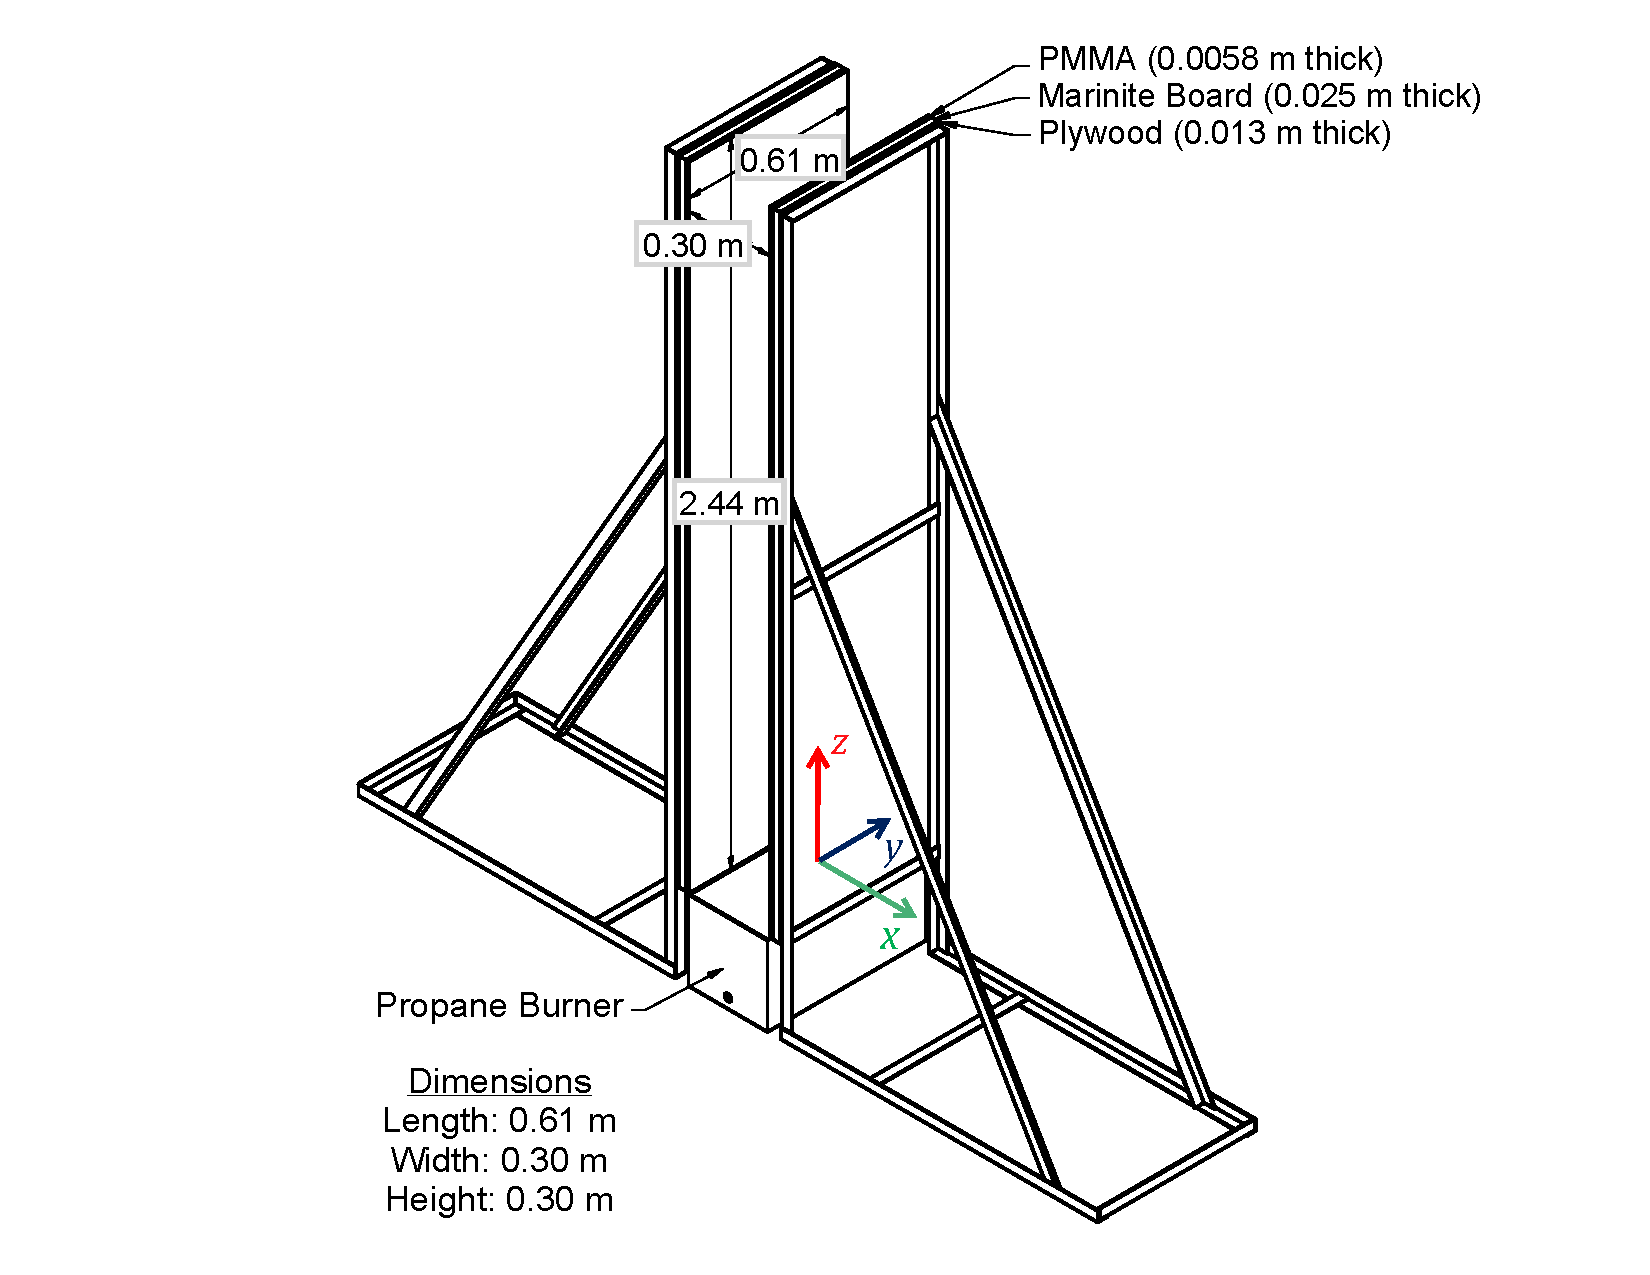
\includegraphics[width=0.75\textwidth]{../../Fire_Growth/NIST_Parallel_Panel/Documentation/Panel_Assembly.pdf}
         \caption{Schematic of the Parallel Panel Apparatus (original apparatus design based on FM~4910~\cite{FM-4910standard}; tests conducted at NIST)}
         \label{fig:Panel_Schematic}
\end{figure}


\vskip.5\baselineskip
\noindent Model setup guidelines:
\vskip.2\baselineskip
\noindent Suggested grid resolution: $\Delta x$ from 0.25~cm to 1~cm.
\vskip.2\baselineskip
\noindent Suggested angular resolution: $N_{\Omega}$ = 100 angles.

\newpage
Groups are invited to first perform a simulation of the heat transfer induced by the propane burner flame to inert Marinite walls, without the PMMA plates. Plots of interest include:
\begin{itemize}[noitemsep]
\item A plot showing the time variations of the heat release rate;
\item Representative plots showing the instantaneous flame shape (e.g., identified as the 200~kW~m$^{-3}$ iso-contour of the volumetric heat release rate, or using some other method to be specified);
\item Plots showing the time variations of the total gauge heat flux (measured by a water cooled sensor) on the surface of one of the two Marinite boards, at a central position ($y = 0$), and for different elevations $z$;
\item Plots showing the spatial variations of the total gauge heat flux (measured by a water cooled sensor) obtained at steady state on the surface of one of the two Marinite boards, for different horizontal positions $y$, and for different elevations $z$.
\end{itemize}

Groups are invited to then perform a simulation with the PMMA plates. Plots of interest include:
\begin{itemize}[noitemsep]
\item A plot showing the time variations of the heat release rate;
\item A plot showing the time variations of the total heat flux measured as a distant location (at $x =$~-1~m, $y =$~-3~m, and $z =$~0.9~m); (note: this heat flux gauge is oriented horizontally, facing towards the gap between the two panels [i.e., pointing towards $x =$~0~m, $y =$~-0.3~m, and $z =$~0.9~m])
\item Representative plots showing the instantaneous flame shape (e.g., identified as the 200~kW~m$^{-3}$ iso-contour of the volumetric heat release rate, or using some other method to be specified);
\item Plots showing the time variations of the total gauge heat flux (measured by a water-cooled sensor) on the surface of one of the two PMMA plates, at a central position ($y = 0$), and for different elevations $z$;
\item Similar plots showing the vertical variations of the total gauge heat flux (measured by a water-cooled sensor) on the surface of one of the two PMMA plates, at a central position ($y = 0$), and for different values of the heat release rate, HRR = 120, 200, 300, 400, 510, 750, 990, 1500, 1980, 2800~kW;
\item Plots showing the vertical variations of the fuel mass loss rate, the surface temperature, the net surface heat flux, and the convective and radiative components of the net surface heat flux on the surface of one of the two PMMA plates, at a central position $y$, and at times corresponding to different values of the heat release rate, HRR = 120, 200, 300, 400, 510, 750, 990, 1500, 1980, 2800~kW.
\item Plots showing the variations of the mean and rms gas temperature along the direction normal to one of the two PMMA plates, at a central position $y$, at vertical elevations $z =$~50~cm, 140~cm and 220~cm, and at times corresponding to different values of the heat release rate, HRR = 120, 300, 750, 1500, 2800~kW.
\item Plots showing the variations of the mean and rms vertical flow velocity along the direction normal to one of the two PMMA plates, at a central position $y$, at vertical elevations $z =$~50~cm, 140~cm and 220~cm, and at times corresponding to different values of the heat release rate, HRR = 120, 300, 750, 1500, 2800~kW.

\end{itemize}


\clearpage
\section{Communicating Results}
\label{Sec:Com-Results}
\subsection{How to Submit Your Results}
Experimental and Modeling Results will be submitted, stored, and made publicly available in the appropriate folders and subfolders of the \href{https://github.com/MaCFP/}{MaCFP GitHub Repository}. Participants can submit their contributions by creating a pull request on Github. For simplicity, please organize all model simulation results for a given target case (see Sec.~\ref{Sec:MaCFP-3 Target Cases}) in a single folder with your INSTITUTE name.  Template files (e.g., .json files holding material property information; .csv files holding results of numerical simulations; and .md files describing simulation setup and results) for all requested numerical simulations results to be provided in these folders are available on the Github repository. Please ensure that your results are formatted as per the guidelines below. Further details on how to contribute are available on the \href{https://github.com/MaCFP/macfp-db/wiki/How-to-Contribute}{MaCFP-db wiki}.

\subsection{Modeling Results: Calibrated Material Property Datasets; (.json files)}

Material property data will be stored in JavaScript Object Notation (JSON) files. JSON is a relatively simple text format for organizing data that has the advantage of being human-readable yet easily parsed in most programming languages. The JSON files characterize a material property dataset in terms of six top level categories characterizing (1) the material, (2) the lab that determined the properties, (3) the details of the calibration procedures used to obtain the properties, (4) the kinetic properties, (5) the thermodynamic properties, and (6) the transport properties.

All of the material properties obtained for the cast black MaCFP PMMA are stored in the MaCFP GitHub repository in the \href{https://github.com/MaCFP/matl-db/tree/master/PMMA/Material_Properties}{Material\_Properties section}. These JSON files provide all of the necessary information to use a particular material property set for predicting the pyrolysis of the MaCFP PMMA. These files are also convenient templates for submitting new material property datasets.

\subsection{Simulations of Fire Behavior and Description of Model Setup (.csv and README.md files)}
Numerical simulations results should be organized in simple ASCII comma-delimited files (.csv files) with clear header names in a format that matches the experimental measurements on the Github Repository. Note: For all submitted results, please confirm that output data is provided using the same file format, data structure (order of data in columns AND data acquisition/output frequency), naming convention (file and data column header names), and reported units as available validation data (see descriptions of available datasets in Sections~\ref{Sec:Gas Phase}, \ref{Sec:Pyrolysis}, and \ref{Sec:Fire Growth}).

Following these standard processing steps (i.e., requiring standard data formatting, units, and naming conventions) is crucial to the success of the MaCFP effort (e.g., standard formatting is necessary to enable the generation and use of scripts for automated processing and comparison of final datasets). This is critical to efficiently analyzing the large number of contributions from participating institutions. Note, some iteration on formatting may be required before the results can be merged into the MaCFP database. If there is ambiguity in the requested file formatting or if you otherwise have questions along these lines, please let us know.

For all modeling cases of interest, researchers must clearly communicate key information regarding how models were setup and run (i.e., descriptions of how results were obtained). This README should be submitted as a markdown file with the information requested \href{https://github.com/MaCFP/macfp-db/blob/master/Utilities/model_questionnaire.md}{on the Modeling Questionnaire} (e.g., contributors, CFD package, submodels \& parameters used, and resolution).

\section{Summary}
\label{Sec:Summary}
The MaCFP-3 Workshop will be held in Tsukuba, Japan, on October 22, 2023. This document provides guidelines for participating in this workshop and submitting modeling results. A highlight of key requests to participants is provided below.\\

\textbf{Gas Phase:}\\
Two experiments of gas-phase fire behavior (liquid pool fires \& gaseous burners, and a co-flow round diffusion flame) are provided for consideration in the MaCFP-3 Workshop. Modelers are asked to provide simulations of one or both of these experiments targeting the specific measurement data presented in Sec.~\ref{Sec:Gas Phase}. Final submissions should be provided by August 31, 2023\\

\textbf{Condensed Phase:}\\
New data has been provided for validation of pyrolysis models (i.e., material property sets) submitted to the MaCFP-2 Workshop. Condensed-phase modelers are asked to submit new predictions of material response to these test conditions (well-characterized radiant heating in an anaerobic environment) using their original MaCFP-2 pyrolysis models. If sufficient agreement is not observed, modelers are asked to recalibrate their property sets (new models are also welcomed). However, we emphasize the need to use independent model calibration and model validation datasets: for this exercise, pyrolysis models should $not$ be directly calibrated to new validation data.  

Although no limitations are provided regarding pyrolysis model calibration approach, all submitted models are required to use either (a) at least one of the milligram-scale datasets (e.g., TGA or DSC) and one gram- scale experiment (e.g., cone calorimetery or controlled atmosphere gasification experiments), or (b) at least two of the gram-scale experiments available in the \href{https://github.com/MaCFP/matl-db/tree/master/PMMA/Calibration_Data}{Calibration\_Data section} of the MaCFP repository. Modelers can supplement MaCFP data with any literature data that they deem necessary. 

Modelers are asked to provide (a) simulations of validation experiments using MaCFP-2 property sets and (b) if needed, to provide updated material property datasets (if needed) by June 1, 2023. These updated material property datasets will be shared (and their predictive accuracy assessed) with the community in a virtual meeting (mid-summer, 2023).\\

\textbf{Coupled Condensed- and Gas-Phase:}\\
New measurement data has been provided for validation of fire growth simulations (flame spread over MaCFP-PMMA; a coupled condensed- and gas-phase scenario). Specifically, HRR, wall flame heat flux, and heat flux at a distance were recorded during upward flame spread over (a) 1.46~m tall PMMA walls in a corner configuration and (b) 2.44~m tall PMMA walls in a parallel panel configuration.
Modelers are asked to provide simulations of one or both of these experiments using material property sets developed by the participants of the condensed-phase portion of this working group. Final submissions should be provided by August 31, 2023. 

\section{Contact Information}
 \subsection*{MaCFP Virtual Discussion Forum}
A Google Discussion Group for the MaCFP Working Group can be accessed online at: \url{https://groups.google.com/g/macfp-discussions/}. The purpose of this Forum is to help develop the network between fire research scientists, to provide a community-wide forum for discussion and exchange of information, and to facilitate data sharing and model development to improve computational predictions of fire behavior.\\

 \subsection*{Additional Points of Contact}
\noindent For general questions on MaCFP, please contact Bart Merci (\href{mailto:bart.merci@ugent.be}{bart.merci@ugent.be}) and Arnaud Trouv\'e (\href{mailto:atrouve@umd.edu}{atrouve@umd.edu}).\\

\noindent For questions on the organization, use, and maintenance of the GitHub MaCFP repository, please contact Randy McDermott (\href{mailto:randall.mcdermott@nist.gov}{randall.mcdermott@nist.gov}).\\

\noindent For questions on specific target experiments, please use the following points of contact:
\begin{table}[htb]
\begin{tabular}{|p{0.6\linewidth} | p{0.4\linewidth}|}
\hline
NIST-Pool-Fires           & Anthony Hamins\\
(Liquid pool fires and gaseous burner experiments)& \href{mailto:anthony.hamins@nist.gov}{anthony.hamins@nist.gov}\\
&\\
\hline
FM-Burner & Yi Wang\\
(Controlled co-flow round diffusion flame experiments)& \href{mailto:yi.wang@fmglobal.com}{yi.wang@fmglobal.com}\\
&\\
\hline
NIST-Gasification-Apparatus & Isaac Leventon \\
(Benchmark gasification experiments of MaCFP-PMMA)&\href{mailto:isaac.leventon@nist.gov}{isaac.leventon@nist.gov}\\
&\\
\hline
UMD-SBI & Stanislav Stoliarov \\
(Flame spread experiments in a 1.46-m tall corner wall &\href{mailto:stolia@umd.edu}{stolia@umd.edu}\\
configuration; based on EN13823~\cite{EN-13823standard})&\\
&\\
\hline
NIST-Parallel-Panel &Isaac Leventon \\
(Flame spread experiments in a 2.44-m tall parallel panel&\href{mailto:isaac.leventon@nist.gov}{isaac.leventon@nist.gov}\\
configuration; based on FM4910~\cite{FM-4910standard})& \\
& \\
\hline

\end{tabular}
\end{table}

\clearpage
\bibliography{../MaCFP_References.bib}

\end{document}
